\chapter{A Dual Chamber Pacemaker Specification}

\begin{itemize}
	\item What are the basic functions?
   \item What happens if new functionality are applied to the basic model?
\end{itemize}
The software component of medical devices are becoming more and more complex. Problems may arise when adding new functionality to already verified software. In this chapter we demonstrate the basic specification of a dual chamber pacemaker, as well as a mode-switch function on top of the basic functions. The specifications are based on the algorithm description in \cite{compass}.
\section{Basic Specifications of a DDD Pacemaker}


%\begin{itemize}
%	\item What are the basic functions?
%   \item What happens if new functionality are applied to the basic model?
%\end{itemize}

\section{Basic Specifications}

The DDD pacemaker has 5 basic timing cycles triggered by external and internal events, as shown in \figref{PMtimers}. We decomposed our pacemaker model into 5 components which correspond to the 5 timers. $P=LRI\| AVI\| URI\| PVARP\| VRP$. These components synchronize with each other using broadcast channels and shared variables (as shown in \figref{PMdesign}). 

\subsection{Lower Rate Interval (LRI)}
%\vspace{-5pt}
The Lower Rate Interval (LRI) component is shown in \figref{PMdesign}(a). This component defines the longest interval allowed between two ventricular events, thus keeping the heart rate above a minimum value. In DDD mode, the LRI interval is divided into a V-A interval (TLRI-TAVI) and a A-V interval (TAVI). The LRI component maintains a maximum V-A delay while the AVI component maintains a maximum A-V delay so together they maintain the maximum V-V delay. In the LRI component, the clock is reset when a ventricular event \textsf{(VS, VP)} is received. If no atrial event has been sensed \textsf{(AS)}, the component will deliver atrial pacing \textsf{(AP)} after TLRI-TAVI. The UPPAAL design of LRI component is shown in \figref{PMdesign}(a).

%\vspace{-5pt}
\subsection{Atrio-Ventricular Interval (AVI) and Upper Rate Interval (URI)}
%\vspace{-5pt}
The function of the AVI component is to maintain the appropriate delay between the atrial activation and the ventricular activation. It defines the longest interval between an atrial event and a ventricular event. If no ventricular event has been sensed \textsf{(VS)} within TAVI after an atrial event \textsf{(AS, AP)}, the component will deliver ventricular pacing \textsf{(VP)}. In order to prevent the pacemaker from pacing the ventricle too fast, a URI component uses a global clock \emph{clk} to track the time after a ventricular event \textsf{(VS, VP)}. The URI limits the ventricular pacing rate by enforcing a lower bound on the times between consecutive ventricle events. If the global clock value is less than TURI when the AVI component is about to deliver \textsf{VP}, AVI will hold VP and deliver it after the global clock reaches TURI. The UPPAAL design of AVI and URI component is shown in \figref{PMdesign}(b) and (c).%The UPPAAL design of AVI component is shown in 

%\vspace{-10pt}
\subsection{Post Ventricular Atrial Refractory Period (PVARP) and Post Ventricular Atrial Blanking (PVAB)}
%\vspace{-5pt}
Ventricular events, especially Ventricular Pace (VP) are sometimes so strong that the atrial lead can sense the activation as well. This signal may be falsely recognized as an atrial event and disrupt normal pacemaker function. This scenario is called crosstalk and was discussed in our previous work \cite{vhm_embc11}. In order to prevent this undesired behavior, there is a blanking period (PVAB) followed by a refractory period (PVARP) for the atrial events after each ventricular event \textsf{(VS, VP)}. Atrial events during PVAB are ignored and atrial events during PVARP trigger \textsf{AR!} events which can be used in some advanced diagnostic algorithms. The UPPAAL design of PVARP component is shown in \figref{PMdesign}(d).

%\vspace{-10pt}
\subsection{Ventricular Refractory Period (VRP)}
%\vspace{-5pt}
Correspondingly, the VRP follows each ventricular event \textsf{(VP, VS)} to filter noise and early events in the ventricular channel which could otherwise cause undesired pacemaker behavior. \figref{PMdesign}(e) shows the UPPAAL design of VRP component.


\begin{figure}[!t]
\center
%\vspace{-10pt}
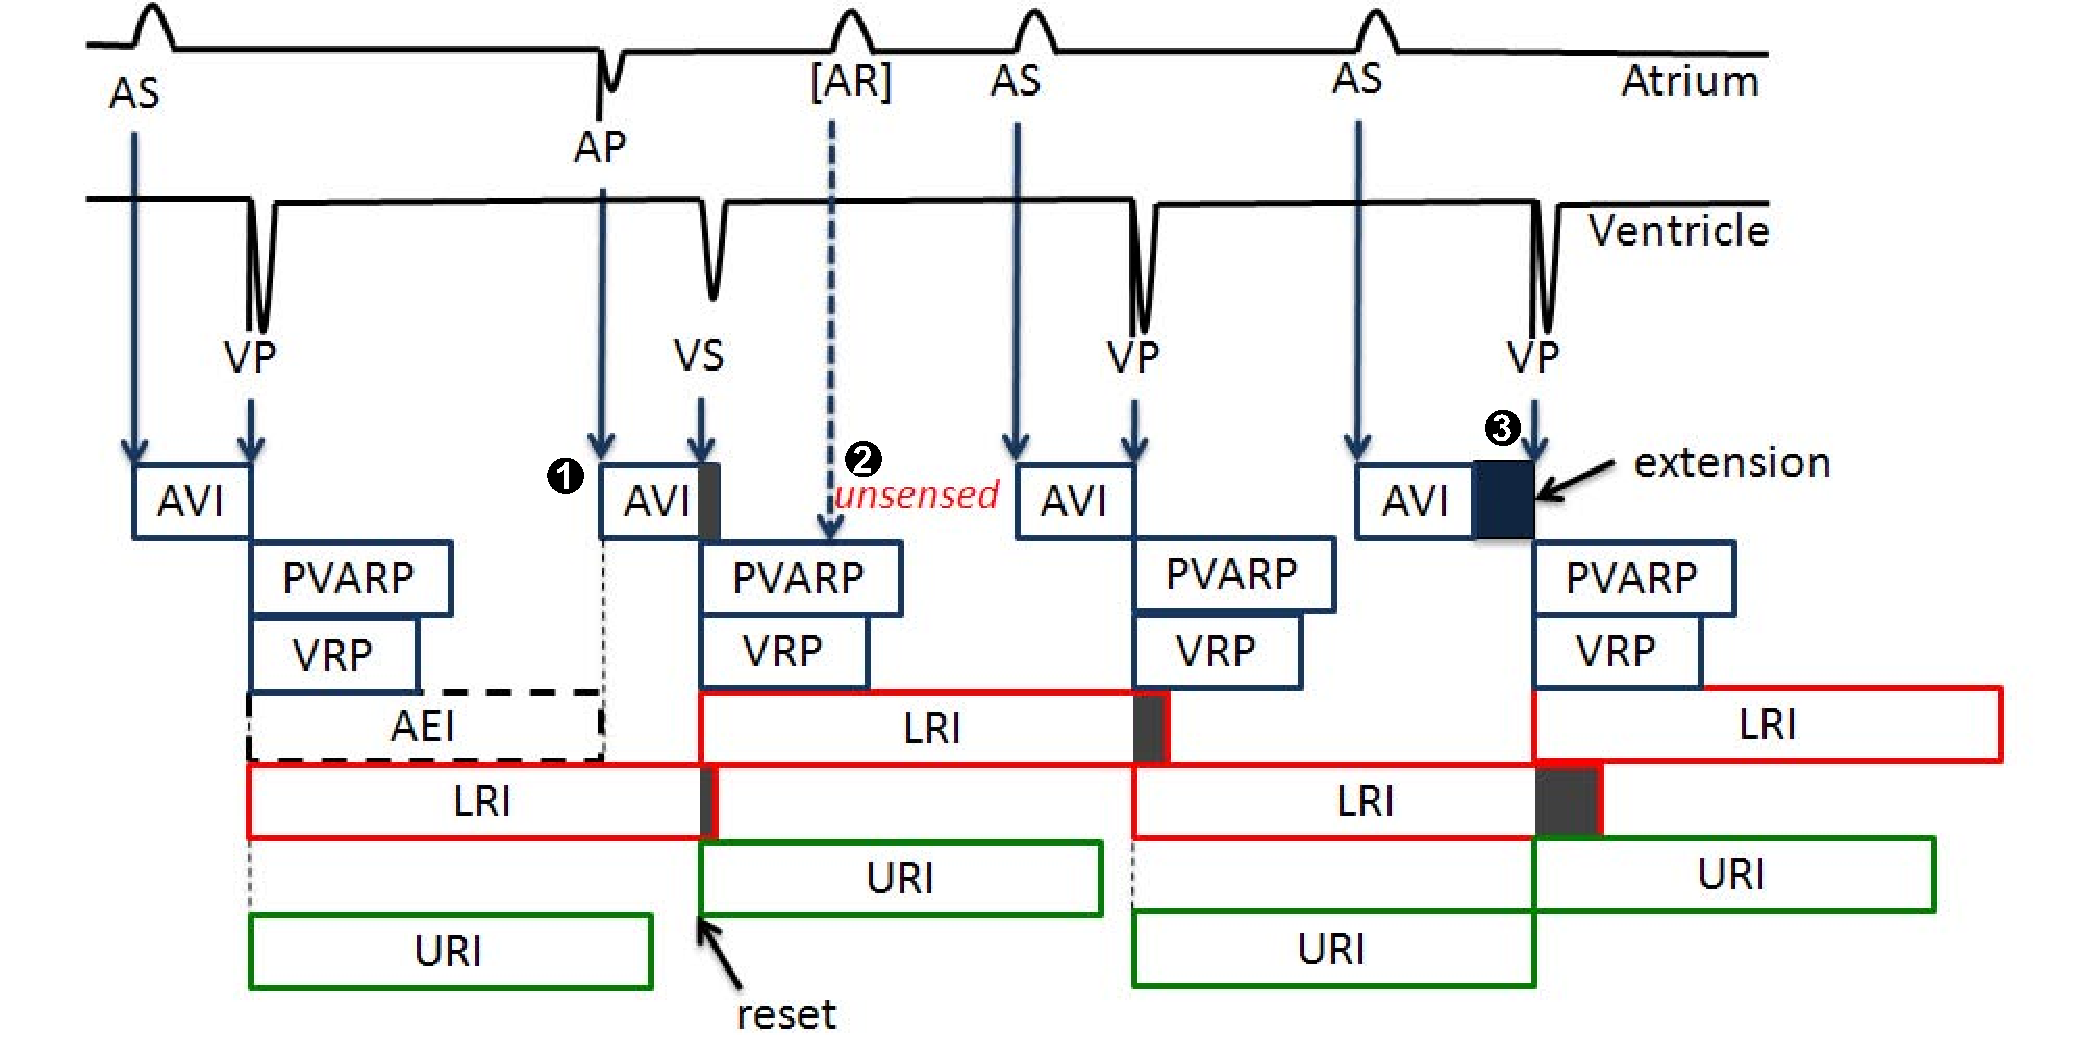
\includegraphics[width=0.7\textwidth]{figs/PM_timers.pdf}
%\vspace{-10pt}
\caption{Basic 5 timing cycles for a dual chamber pacemaker}
\label{fig:PMtimers}
%\vspace{-10pt}t

\end{figure} 
Since the pacemaker operates only on the timing between events. 
\begin{figure}[!t]
\center
%\vspace{-10pt}
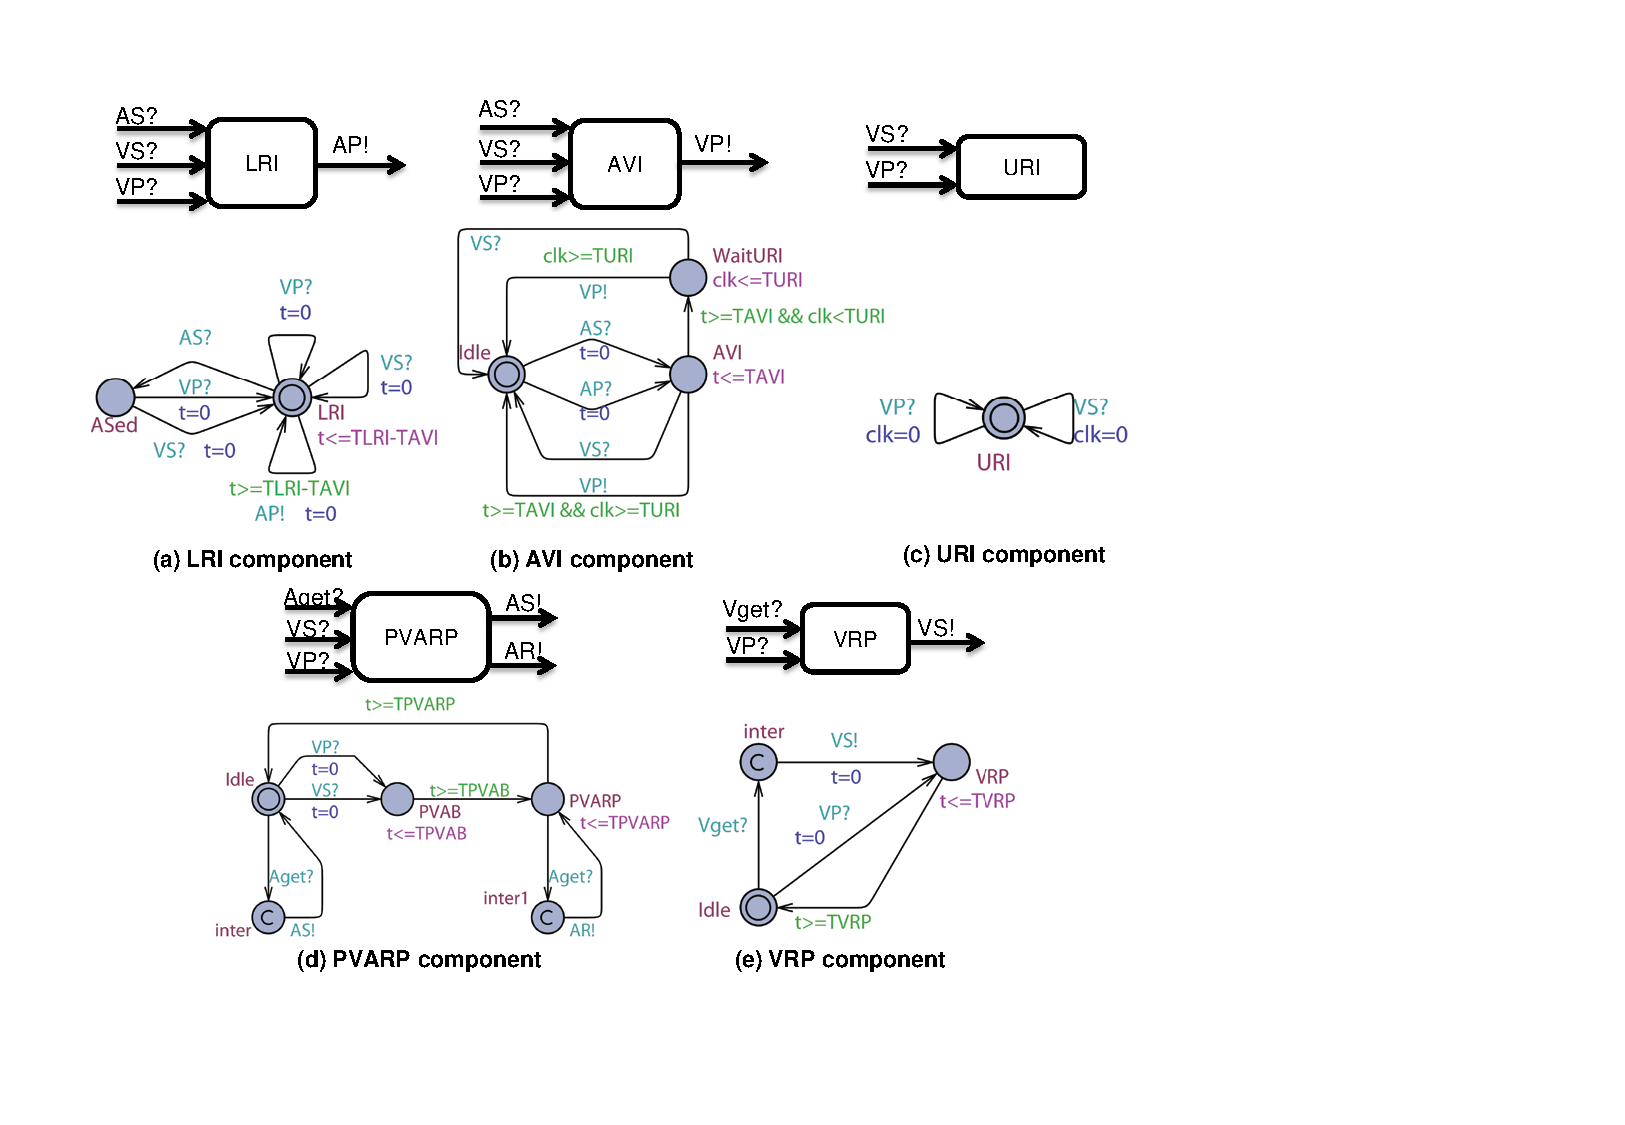
\includegraphics[width=0.9\textwidth]{figs/pacemaker.pdf}
%\vspace{-10pt}
\caption{Basic 5 timing cycles for a dual chamber pacemaker}
\label{fig:PMdesign}
%\vspace{-10pt}
\end{figure} 
\section{Atrial Tachycardia Response (Mode Switch)}
SVT is an arrhythmia which features an abnormally fast atrial rate. %\figref{SVT} is a series of simulation results for closed-loop interaction between a heart model with SVT and the pacemaker model. The atrial and ventricular channels show electrogram inputs to the pacemaker and the pacemaker channel shows the corresponding events received and generated by the pacemaker software, \cite{vhm_embc11}.
Typically, in the open loop case, the AV node, which has a long refractory period, can filter most of the fast atrial activations during SVT thus the ventricular rate remains relatively normal. \figref{SVT_none} demonstrates a pacemaker event trace during SVT, with a ODO mode pacemaker which just sensing in both channels. In this particular case, every 3 atrial events (AS) correspond to 1 ventricular event (VS) during SVT. 
As an arrhythmia, SVT is still considered as a safe heart condition since the ventricles operate under normal rate can and still maintain adequate cardiac output. 

However, in the closed loop case with the pacemaker, the AVI component of a dual chamber pacemaker is equivalent to a virtual pathway in addition to the intrinsic conduction pathway between the atria and the ventricles. The pacemaker tries to maintain 1:1 A-V conduction and thus increases the ventricular rate inappropriately to match the atrial rate. \figref{SVT_DDD} shows the pacemaker trace of the same SVT case with DDD pacemaker. Although half of the fast atrial events are filtered by the PVARP period ([AR]s), the DDD pacemaker still drives the closed-loop system into 2:1 A-V conduction with faster ventricular rate, which is inappropriate. This problem can be resolved by switching the pacemaker from the dual chamber mode, which couples the atrial and ventricular rates, into a single chamber mode to maintain appropriate ventricular rate independent of the atrial rate. 
\begin{figure*}[!t]
\centering
		\subfigure [\small]{			
		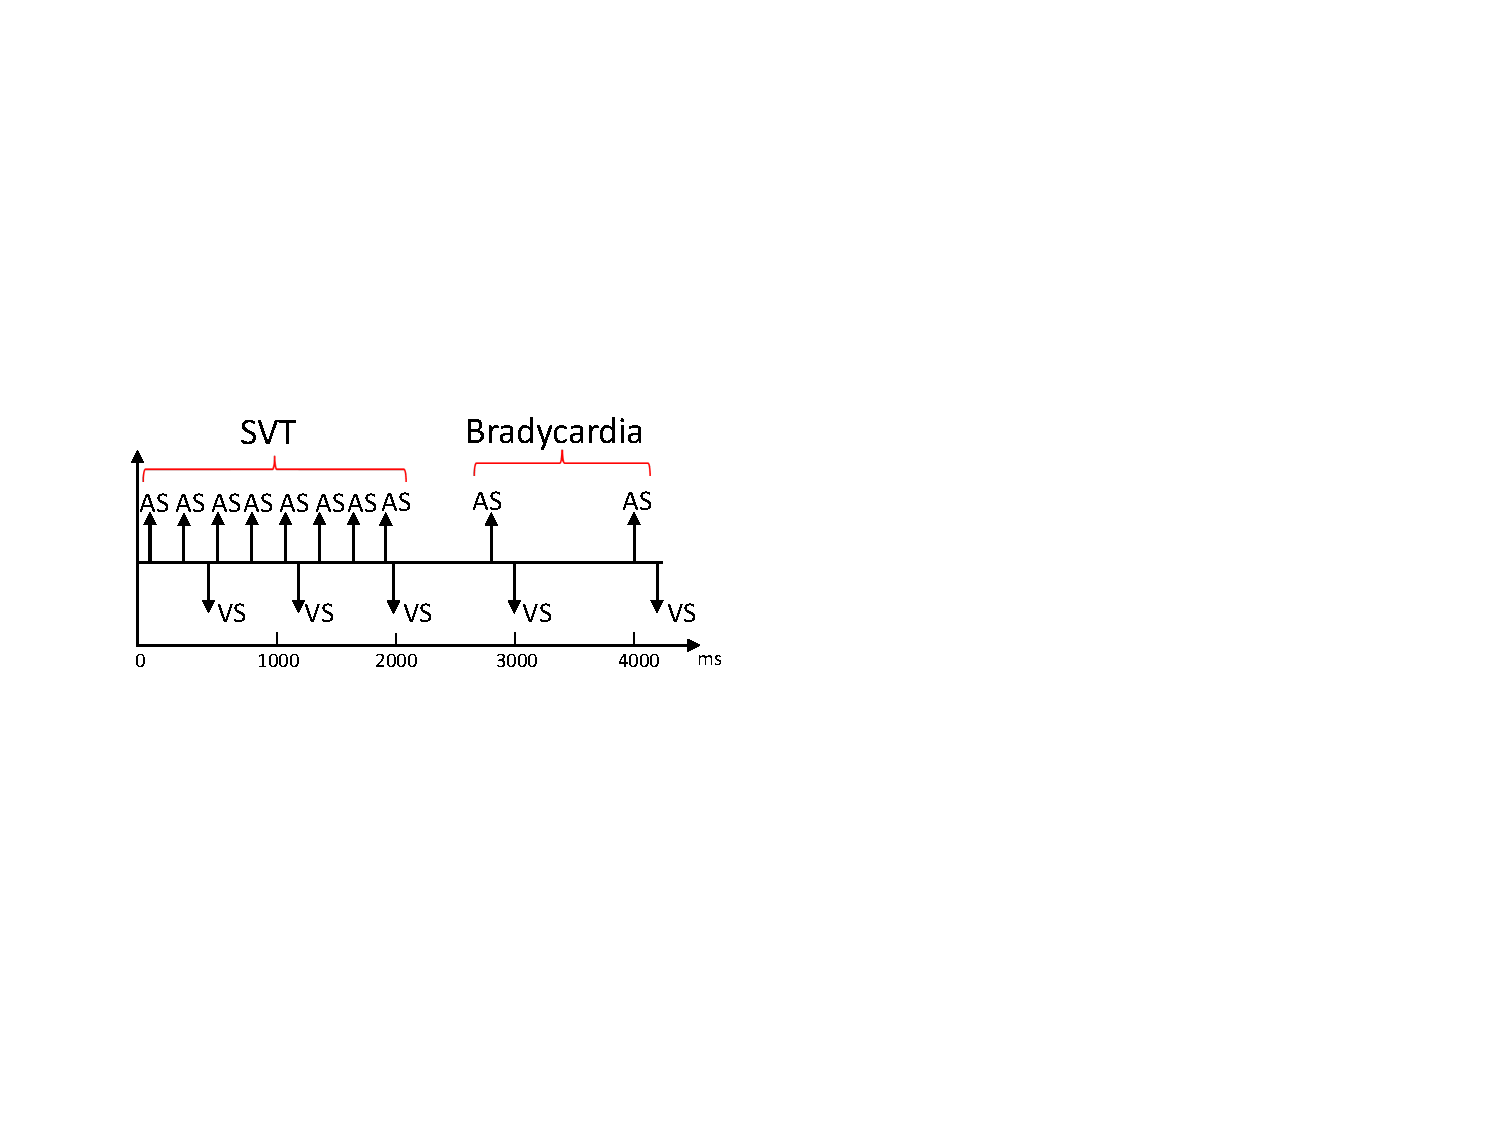
\includegraphics[width=0.4  \textwidth]{figs/SVT_none.pdf}
		\label{fig:SVT_none}
		} 
%	\hspace{.1in}%
		
		\subfigure [\small] 
		{
		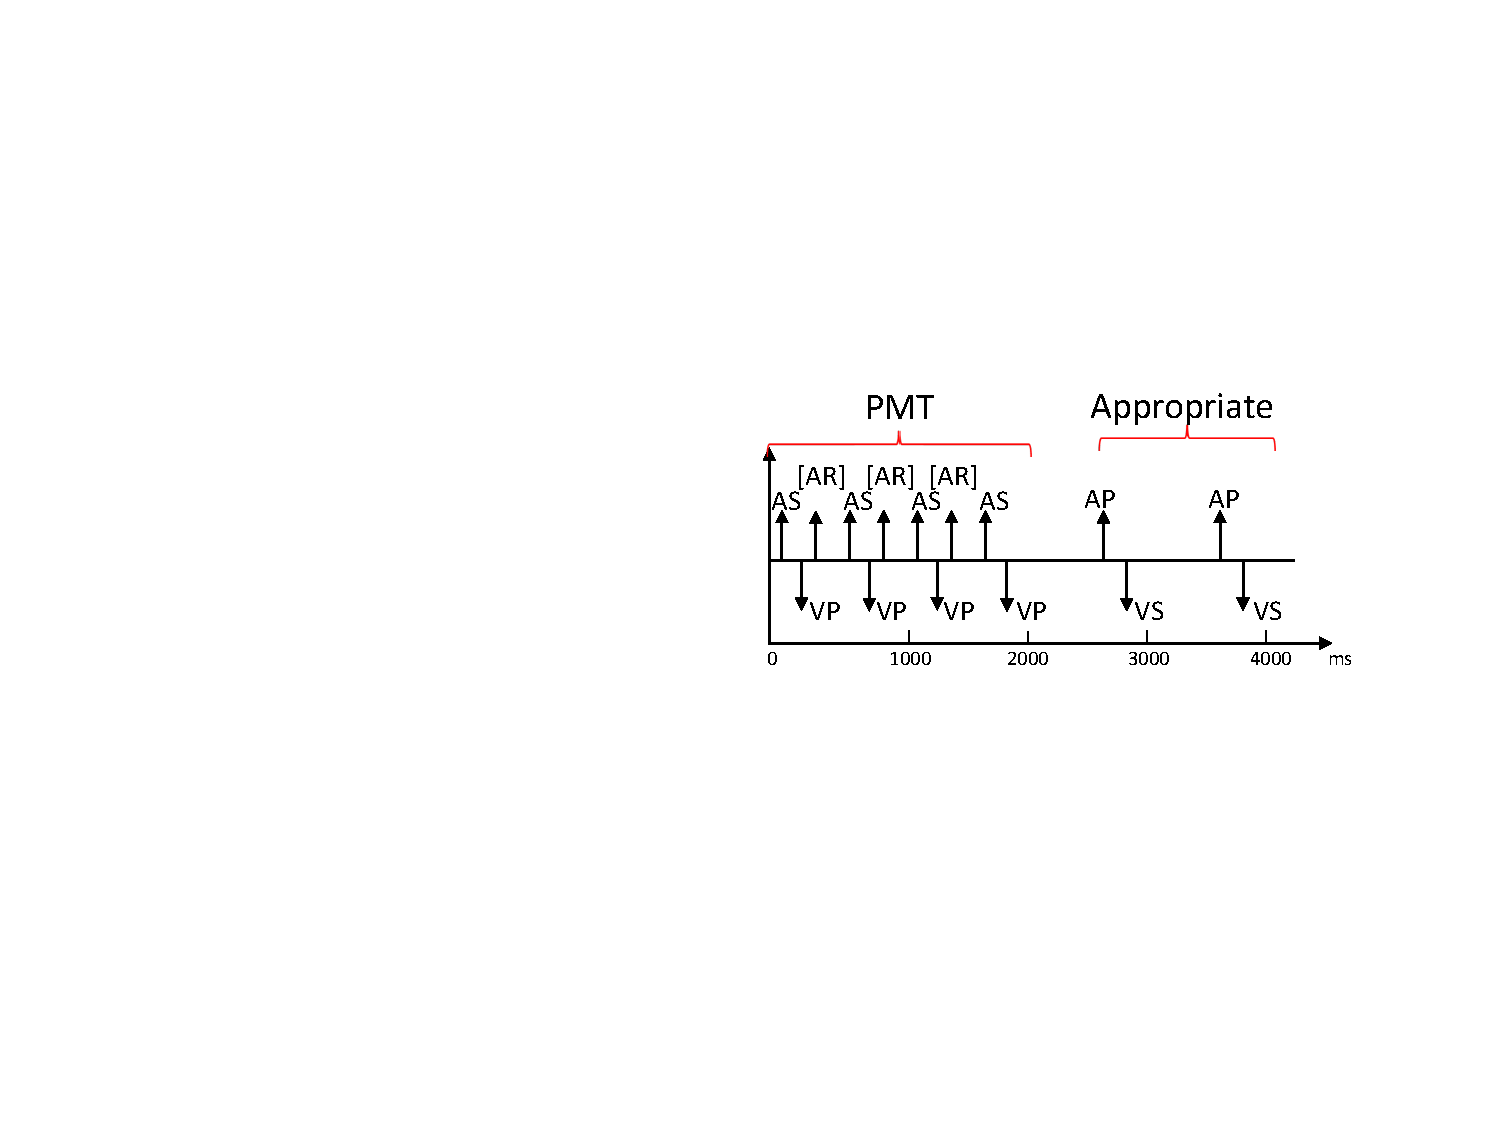
\includegraphics[width=0.4\textwidth]{figs/SVT_DDD.pdf}
		\label{fig:SVT_DDD}
		} 
%\vspace{-10pt}
\caption{\small (a) Node automaton. Dotted transition is only valid for pacemaker tissue like SA node; (b) Path automaton; (c) Model of the electrical conduction system of the heart using a network of node \& path automata~\cite{vhm_ecrts10}.}
%\vspace{-15pt}
\end{figure*} 

We now analyze the approach use in pacemakers to prevent prolonged ventricular pacing under SVT. Intuitively, the mode-switch algorithm first detects SVT. After confirmed detection, it switches the pacemaker from a dual-chamber mode to a single-chamber mode. During the single-chamber mode, the A-V synchrony function of the pacemaker is deactivated thus the ventricular rate is decoupled from the fast atrial rate. After the algorithm determines the end of SVT, it will switch the pacemaker back to the dual chamber mode. 

The mode-switch algorithm specification we use is similar to the one described in the Boston Scientific pacemakers manual \cite{compass}. The algorithm first measures the interval between atrial events outside the blanking period (AS, AR). The interval is considered as \emph{fast} if it is above a threshold (\emph{Trigger Rate}) and \emph{slow} otherwise. In our UPPAAL model we model it as $INT$ (see \figref{dur_count} (1)). A counter $CNT$ increments for \emph{fast} events and decrements for \emph{slow} events (see \figref{dur_count} (2)). After the counter value reaches the \emph{Entry Count}, the algorithm will start a \emph{Duration} ($DUR$) which is a time interval used to confirm the detection of SVT (see \figref{dur_count} (3)). In the \emph{Duration}, the counter keeps counting. If the counter value is still positive after the \emph{Duration}, the pacemaker will switch to the VDI mode (\emph{Fallback mode}). In the VDI mode, the pacemaker only senses and paces the ventricle. At any time if the counter reaches zero, the \emph{Duration} will terminate and the pacemaker is switched back to DDD mode.
% to show some interesting findings. The basic idea of this simplified model is explained in detail. \\
%\mySubSubSection{UPPAAL model for mode-switch algorithm}
In our UPPAAL model of the mode-switch algorithm, we use nominal parameter values from the clinical setting. We define \emph{trigger rate} at 170bpm (350ms), \emph{entry count} at 8, \emph{duration} for 8 ventricular events and \emph{fallback mode} as VDI. 


In order to model both DDD and VDI modes and the switching between them, we made modifications to the AVI and LRI components.
In each component two copies for both modes are modeled, and switch between each other when switching events (DDD, VDI) are received. During VDI mode, VP is delivered by the LRI component instead of the AVI component. The clock values are shared between both copies in order to preserve essential intervals even after switching. The modified AVI ($AVI'$) and LRI ($LRI'$)components are shown in \figref{avi_ms}. 
\begin{figure*}
		\centering
		%\vspace{-19pt}
		\includegraphics[width=0.8\textwidth]{figs/AVI_ms.pdf}
		%\vspace{-10pt}
		\caption{\small (a) After switching to \textsf{VDI} mode, the new LRI component \textsf{LRI'} maintains a minimum V-V interval; (b) After switching to \textsf{VDI} mode, the new AVI component \textsf{AVI'} keeps track of the time after each atrial events.}
		%  \vspace{-20pt}
		\label{fig:avi_ms}
\end{figure*}
\begin{figure*}
		\centering
				%\vspace{-15pt}
		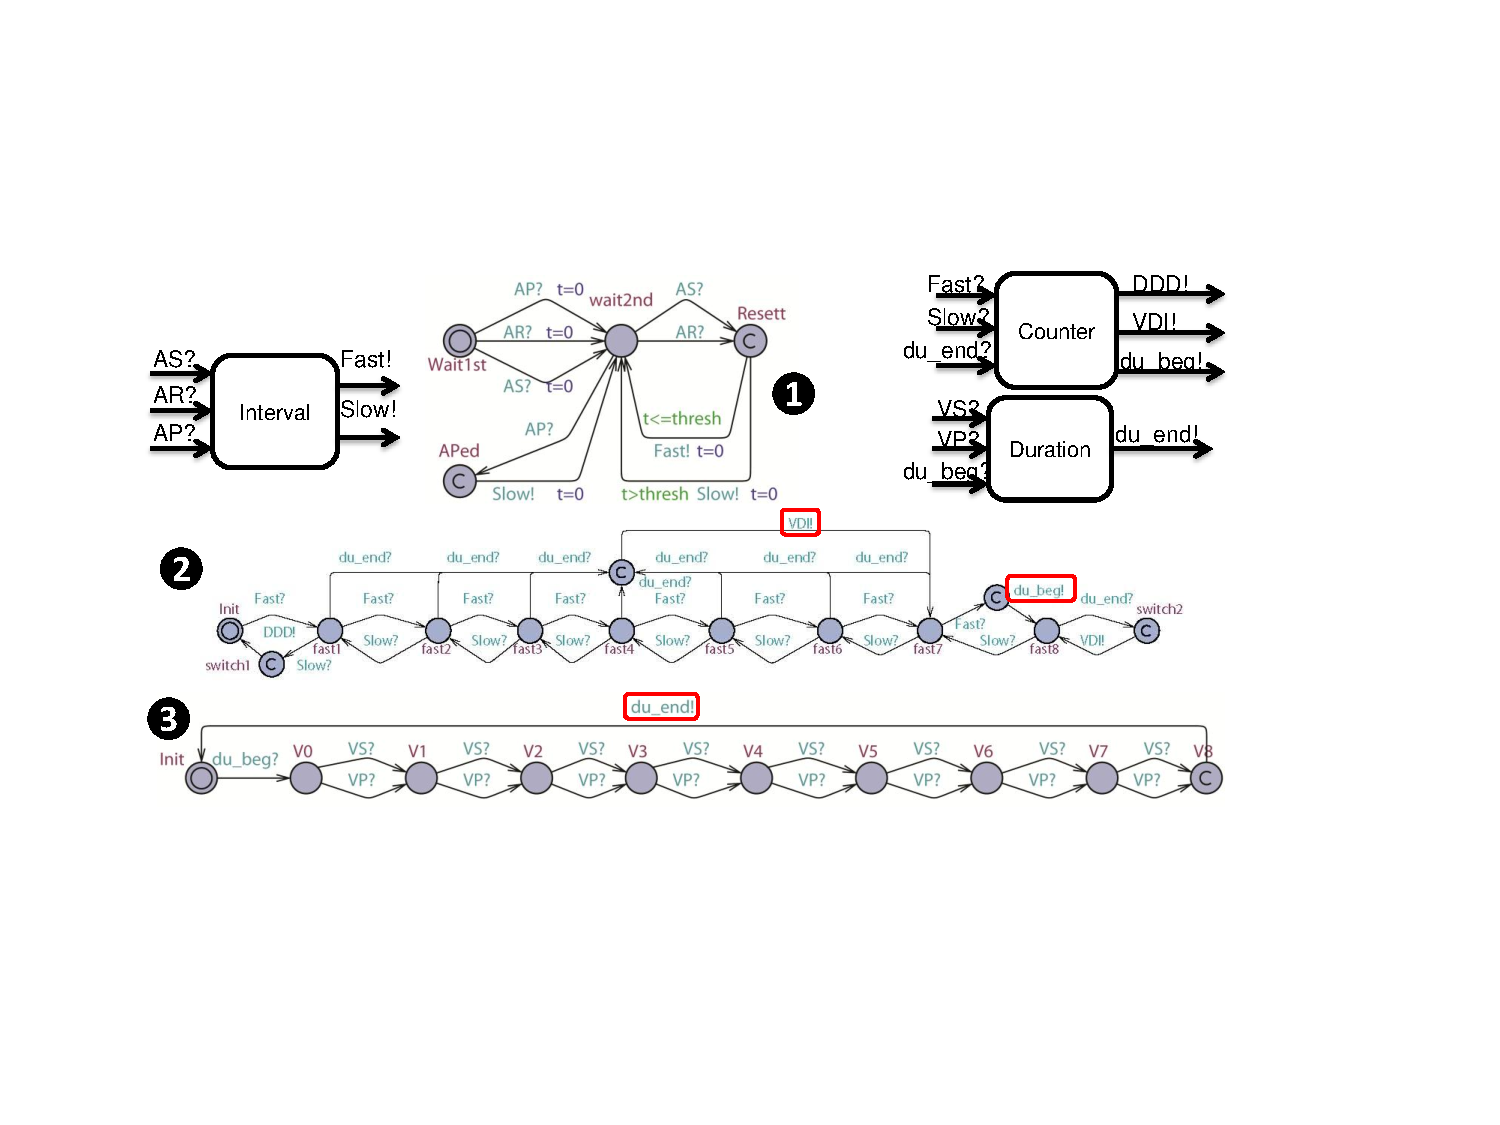
\includegraphics[width=0.9\textwidth]{figs/duration.pdf}
		\vspace{-10pt}
		\caption{\small (a) Component \textsf{INT} An atrial event (\textsf{AS,AR}) arrive before \textsf{thresh} after the previous atrial event is regarded as \textsf{fast} event. Atrial event arrive after \textsf{thresh} and \textsf{AP} are regarded as \textsf{slow} event; (b) Component \textsf{CNT} After 8 \textsf{fast} event the algorithm will start a duration by sending \textsf{du\_beg} and will switch to \textsf{VDI} mode when the duration ends (\textsf{du\_end}); (c) Component \textsf{DUR} The duration length is 8 ventricular events (\textsf{VS,VP})}
		  %\vspace{-15pt}
		\label{fig:dur_count}
\end{figure*} 

\chapter{Closed-loop Model Checking}
\begin{itemize}
	\item How to use models to cover environmental conditions specified in the physiological requirements, that the device may encounter?
            \item Can model checking find violations that testing cannot find?
            \item What are the effects of adding new features to the software? Can they disrupt the safety properties that the previous device hold?
            \item What is the model complexity requirements for each physiological requirement? When and how to refine the environment model?
            \item Exploring the whole state space sounds great. What are the limitations of model checking? 
\end{itemize}
In model-based software design, the system can be abstracted by a model. With proper model formalism and tools, the whole state space of the system can be checked
\begin{figure*}
\centering
%\vspace{-10pt}
		\subfigure[Monitor \textsf{PLRI\_test}] {
				\includegraphics[width=0.5\textwidth]{figs/LRI_test.pdf}
				\label{fig:safety1}
		} 
		\subfigure[Monitor \textsf{PURI\_test}] {	
			\includegraphics[width=0.45\textwidth]{figs/uri_test.pdf}
			\label{fig:uri_test}
		}
		%\vspace{-10pt}
	\caption{(a) Monitor for LRL: Interval between two ventricular events should be less than TLRI, (b) Monitor for URL: Interval between a ventricular event and a VP should be longer than TURI}
%\vspace{-15pt}
\end{figure*} 
\section{Reachability of Unsafe Regions}
The basic function of a pacemaker is to increase heart rate when necessary. As the result, we not only want to verify that the heart rate has been increased accordingly, but also ensure the pacemaker does not increase the heart rate too much. Since these requirements should hold for all possible heart conditions, the most abstract heart model $H_4$ is selected as the environment model. The following two requirements specify the unsafe regions  (too fast and too slow) within the closed-loop state space.

\subsection{Lower Rate Limit}
The most essential function for the pacemaker is to treat bradycardia by maintaining the ventricular rate above a certain threshold. We define the region where the ventricular rate is slow, as \textsf{unsafe}. The monitor \textsf{PLRI\_test} is designed to measure intervals between ventricular events and is shown in \figref{safety1}. For property \\
\textsf{$\varphi_{LRI}=$A[] (PLRI\_test.secV imply PLRI\_test.t$\leq$TLRI)}\\ we have $H_4\| P\| PLRI\_test\models\varphi_{LRI}$.

\subsection{Upper Rate Limit}
The pacemaker is not designed to treat tachycardia so it can only pace the heart to increase its rate and cannot slow it down. However, it is still important to guarantee it does not pace the ventricles beyond a maximum rate to ensure safe operations. To this effect, an Upper Rate Interval (URI) is specified such that the pacemaker can increase the ventricular rate up to this limit. 
  
We require that a ventricle pace (VP) can only occur at least $TURI$ after a ventricle event (VS, VP). The monitor \textsf{PURI\_test} is shown in \figref{uri_test}. For the property\\
$\varphi_{URI}=$\textsf{A[] (PURI\_test.secV imply PURI\_test.t$\geq$TURI)} \\
we have $H_4\| P\| PURI\_test\models \varphi_{URI}$.

\section{Model Checking the Mode-Switch Algorithm}

\subsection{Existence of PMT during SVT}
The monitor \textsf{Pv\_v} is designed to show existence of PMT during SVT. It goes to the error state if the ventricular rate drops below the Upper Rate Limit (\figref{vv}).  
\begin{figure}
		\centering
		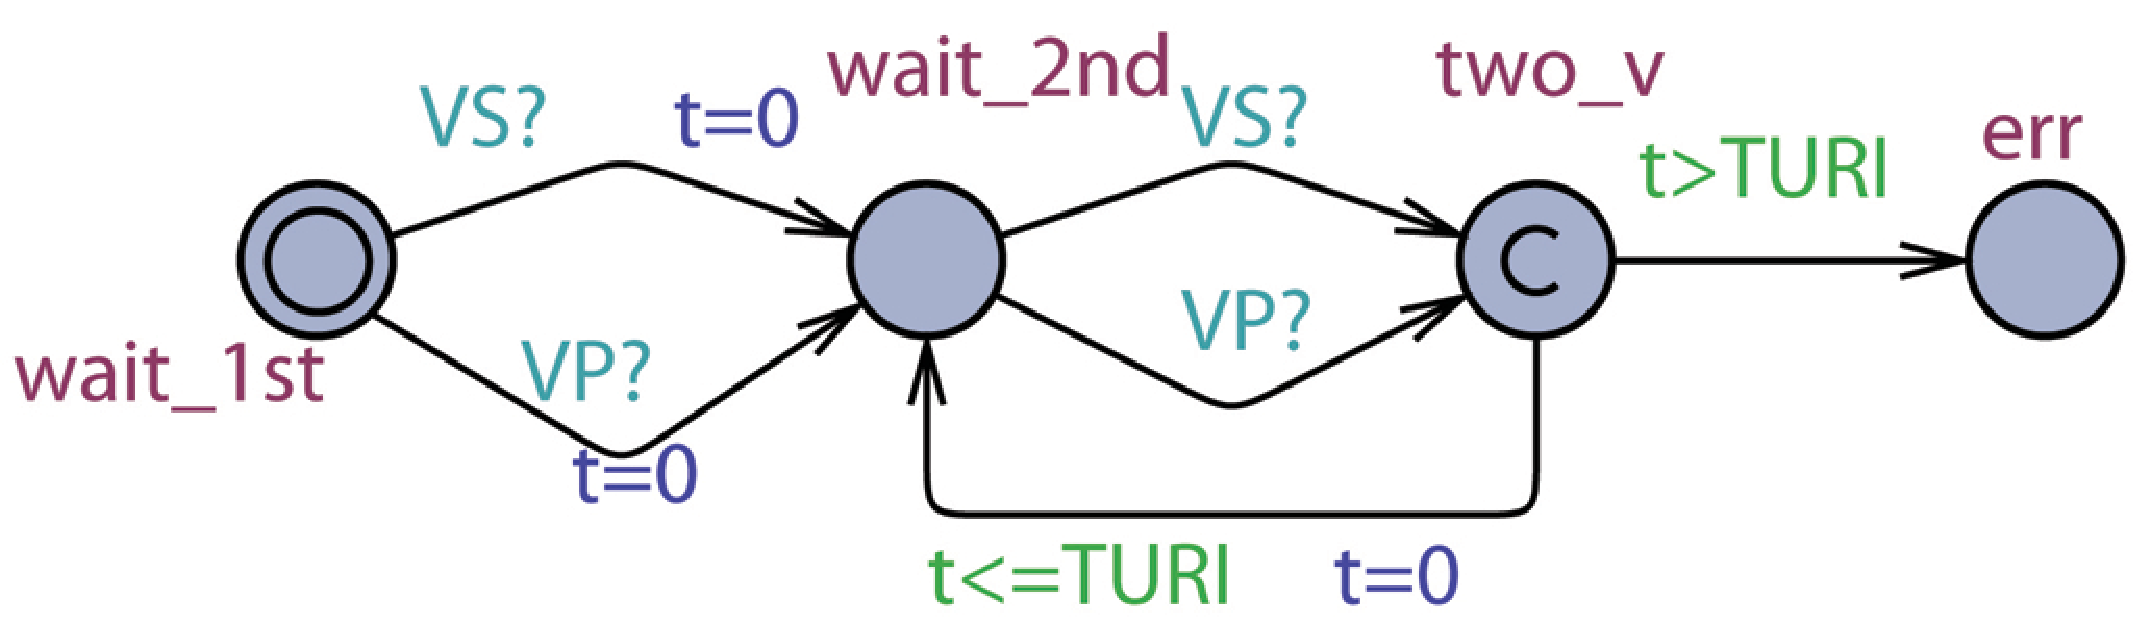
\includegraphics[width=0.4\textwidth]{figs/vv.pdf}
		\caption{\small Monitor \textsf{Pv\_v} for SVT: There exists an endless sequence in which interval between ventricular events is at most TURI}
		  %\vspace{-15pt}
		\label{fig:vv}
\end{figure}

We specify\\
$\varphi_{MS}=E[] (not Pv\_v.err)$\\
which verifies the existence of PMT. The heart model $H_3$ is not suitable for this property since the non-deterministic conduction of component $P_3$ does not capture the blocking property of the AV node, which is the key in PMT. We use a more refined model $H_2$ which has AV node modeled. To identify the PMT scenario, we first set $H_2.N^1.Trest\_min<100$ so that the atrial rate can be high and $H_2.N^2.Trest\_min>TURI$ so that the intrinsic heart rate is less than TURI. The property is first verified on pacemaker without the mode-switch algorithm. We have\\
$H_2\|P\|Pv\_v\models\varphi_{MS}$
and the evidence returned by the model checker illustrates the PMT scenario.

\subsection{Mode-Switch Algorithm}
We now analyze the approach use in pacemakers to prevent prolonged ventricular pacing under SVT. Intuitively, the mode-switch algorithm first detects SVT. After confirmed detection, it switches the pacemaker from a dual-chamber mode to a single-chamber mode. During the single-chamber mode, the A-V synchrony function of the pacemaker is deactivated thus the ventricular rate is decoupled from the fast atrial rate. After the algorithm determines the end of SVT, it will switch the pacemaker back to the dual chamber mode. 

The mode-switch algorithm specification we use is similar to the one described in the Boston Scientific pacemakers manual \cite{compass}. The algorithm first measures the interval between atrial events outside the blanking period (AS, AR). The interval is considered as \emph{fast} if it is above a threshold (\emph{Trigger Rate}) and \emph{slow} otherwise. In our UPPAAL model we model it as $INT$ (see \figref{dur_count} (1)). A counter $CNT$ increments for \emph{fast} events and decrements for \emph{slow} events (see \figref{dur_count} (2)). After the counter value reaches the \emph{Entry Count}, the algorithm will start a \emph{Duration} ($DUR$) which is a time interval used to confirm the detection of SVT (see \figref{dur_count} (3)). In the \emph{Duration}, the counter keeps counting. If the counter value is still positive after the \emph{Duration}, the pacemaker will switch to the VDI mode (\emph{Fallback mode}). In the VDI mode, the pacemaker only senses and paces the ventricle. At any time if the counter reaches zero, the \emph{Duration} will terminate and the pacemaker is switched back to DDD mode.
% to show some interesting findings. The basic idea of this simplified model is explained in detail. \\
%\mySubSubSection{UPPAAL model for mode-switch algorithm}
In our UPPAAL model of the mode-switch algorithm, we use nominal parameter values from the clinical setting. We define \emph{trigger rate} at 170bpm (350ms), \emph{entry count} at 8, \emph{duration} for 8 ventricular events and \emph{fallback mode} as VDI. 


In order to model both DDD and VDI modes and the switching between them, we made modifications to the AVI and LRI components.
In each component two copies for both modes are modeled, and switch between each other when switching events (DDD, VDI) are received. During VDI mode, VP is delivered by the LRI component instead of the AVI component. The clock values are shared between both copies in order to preserve essential intervals even after switching. The modified AVI ($AVI'$) and LRI ($LRI'$)components are shown in \figref{avi_ms}. So the new pacemaker model is:\\
$P_2$=\textsf{LRI'$\|$AVI'$\|$URI$\|$PVARP$\|$VRP$\|$INT$\|$CNT$\|$DUR}
% There are two separate AVI and LRI components for each mode and switches to the corresponding ones when synchronization signals are received. The clock values are kept so that essential intervals are kept. 
\subsection{Verification against fundamental safety properties}
We verify the same fundamental safety properties on the pacemaker model with mode-switch algorithm. We have:
$$H_2\|P_2\|PURI\_test\models\varphi_{URI}$$
$$H_2\|P_2\|PLRI\_test\not\models\varphi_{LRI}$$
The Upper Rate Limit property still holds but the Lower Rate Limit property is violated. The counterexample is proved to be valid after checking the trace of more refined heart models. By analyzing the trace we found that when the pacemaker is switching from VDI mode to DDD mode, the responsibility to deliver VP switched from LRI component to AVI component. Since the clock reference is different (Ventricular events in LRI component and Atrial events in AVI component), the clock value for delivering the next VP is not preserved. As a result, if an atrial event which triggered the mode-switch from VDI to DDD happens within [TLRI-TAVI, TLRI) after the last ventricular event, the next ventricular pacing will be delayed by at most TAVI time, which violates the Lower Rate Limit property (\figref{safety}). 
\begin{figure}
		\centering
		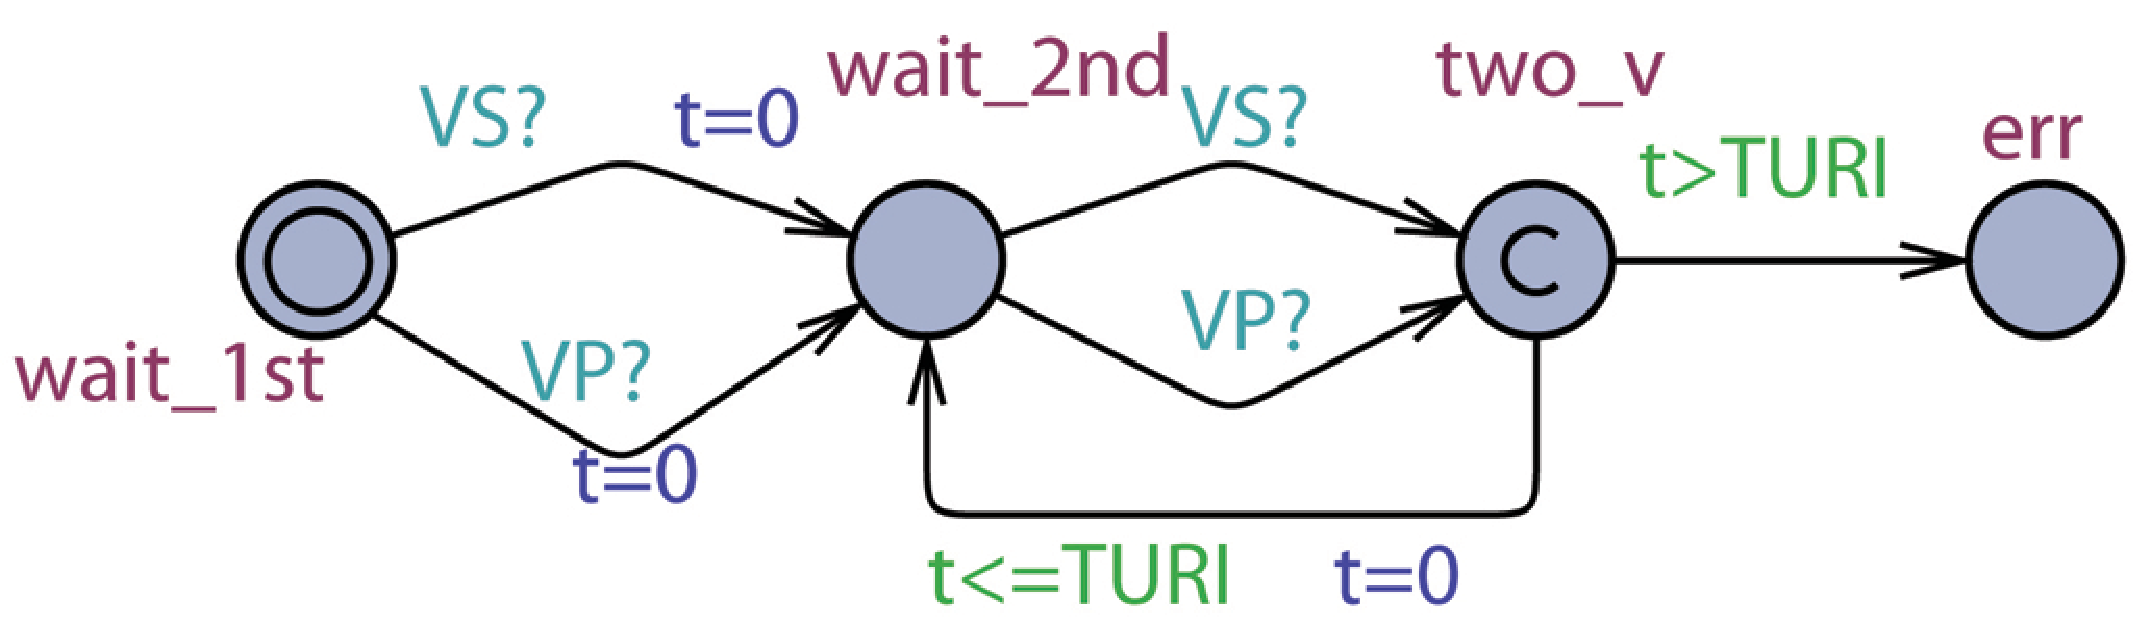
\includegraphics[width=0.4\textwidth]{figs/vv.pdf}
		\caption{\small Monitor \textsf{Pv\_v} for SVT: There exists an endless sequence in which interval between ventricular events is at most TURI}
		  %\vspace{-15pt}
		\label{fig:vv}
\end{figure}
\subsection{Verification Result}
After implementing the Mode-switch algorithm, we verified the model against the same existence property. We expect the violation of this property, since during VDI mode the ventricular rate of the heart model is less than the Upper Rate Limit and will not trigger ventricular pacing. However, this property is still satisfied, indicating the mode-switch algorithm failed to eliminate the PMT scenario. The evidence trace returned by UPPAAL shows that a subset of atrial events fall into the blanking period after a ventricular event (see \figref{liveness}). As a result, two fast events are reduced to one slow event and mode switch may never happen. This scenario does exist in all our refined heart models, we conclude that the trace is physiologically feasible. The mode-switch algorithm in our pacemaker model can not terminate all PMT behaviors as specified.

\subsection{Trace Validation on Real Pacemaker and Pacemaker Refinement}
In the previous subsections, we have found two potential safety violations in our pacemaker model. However, this does not mean the actual pacemaker has the same violation. Jiang et al. have implemented the VHM model onto a programmable integrated circuit (FPGA) platform and had it interact with a real pacemaker at run-time \cite{PVS}. The closed-loop behavior can be checked in closed-loop with a real pacemaker. If the trace is not feasible in the closed-loop system, the pacemaker model needs to be refined to eliminate the execution. However, refining the pacemaker model requires more detailed representation of the pacemaker software, which was not available to us at that time.
\begin{figure}
\centering
%\vspace{-20pt}
		\subfigure []{
				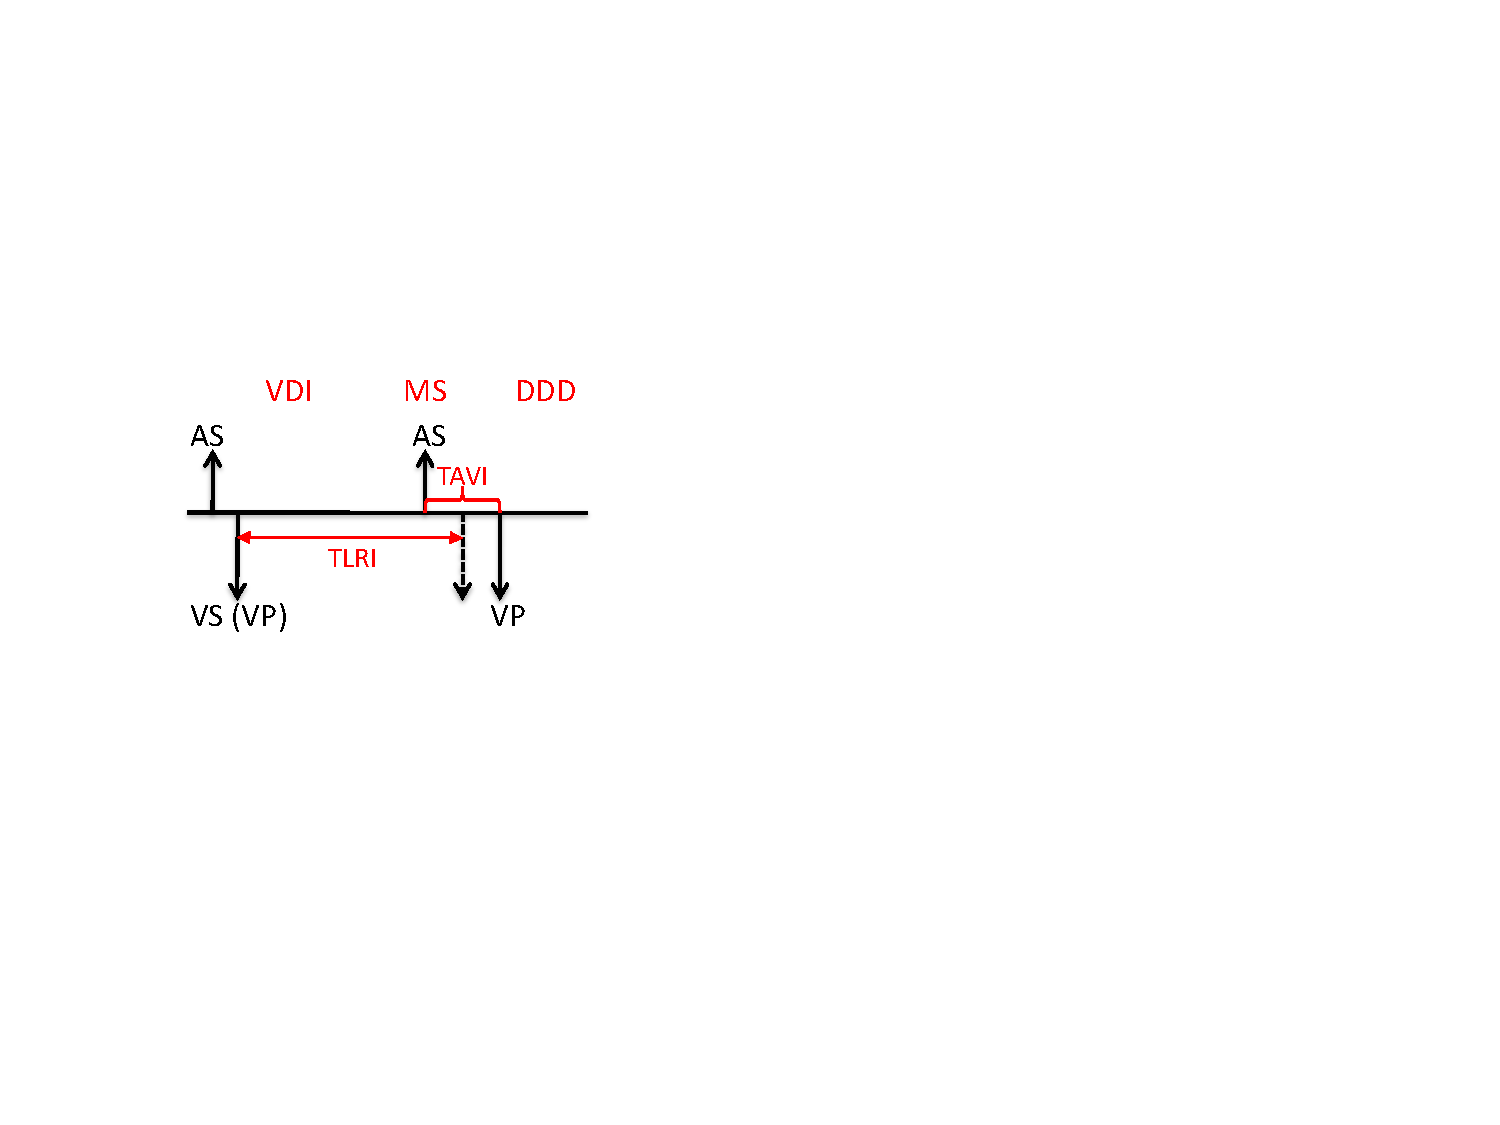
\includegraphics[width=0.2\textwidth]{figs/safety.pdf}
				\label{fig:safety}
		} 
		\subfigure []{	
			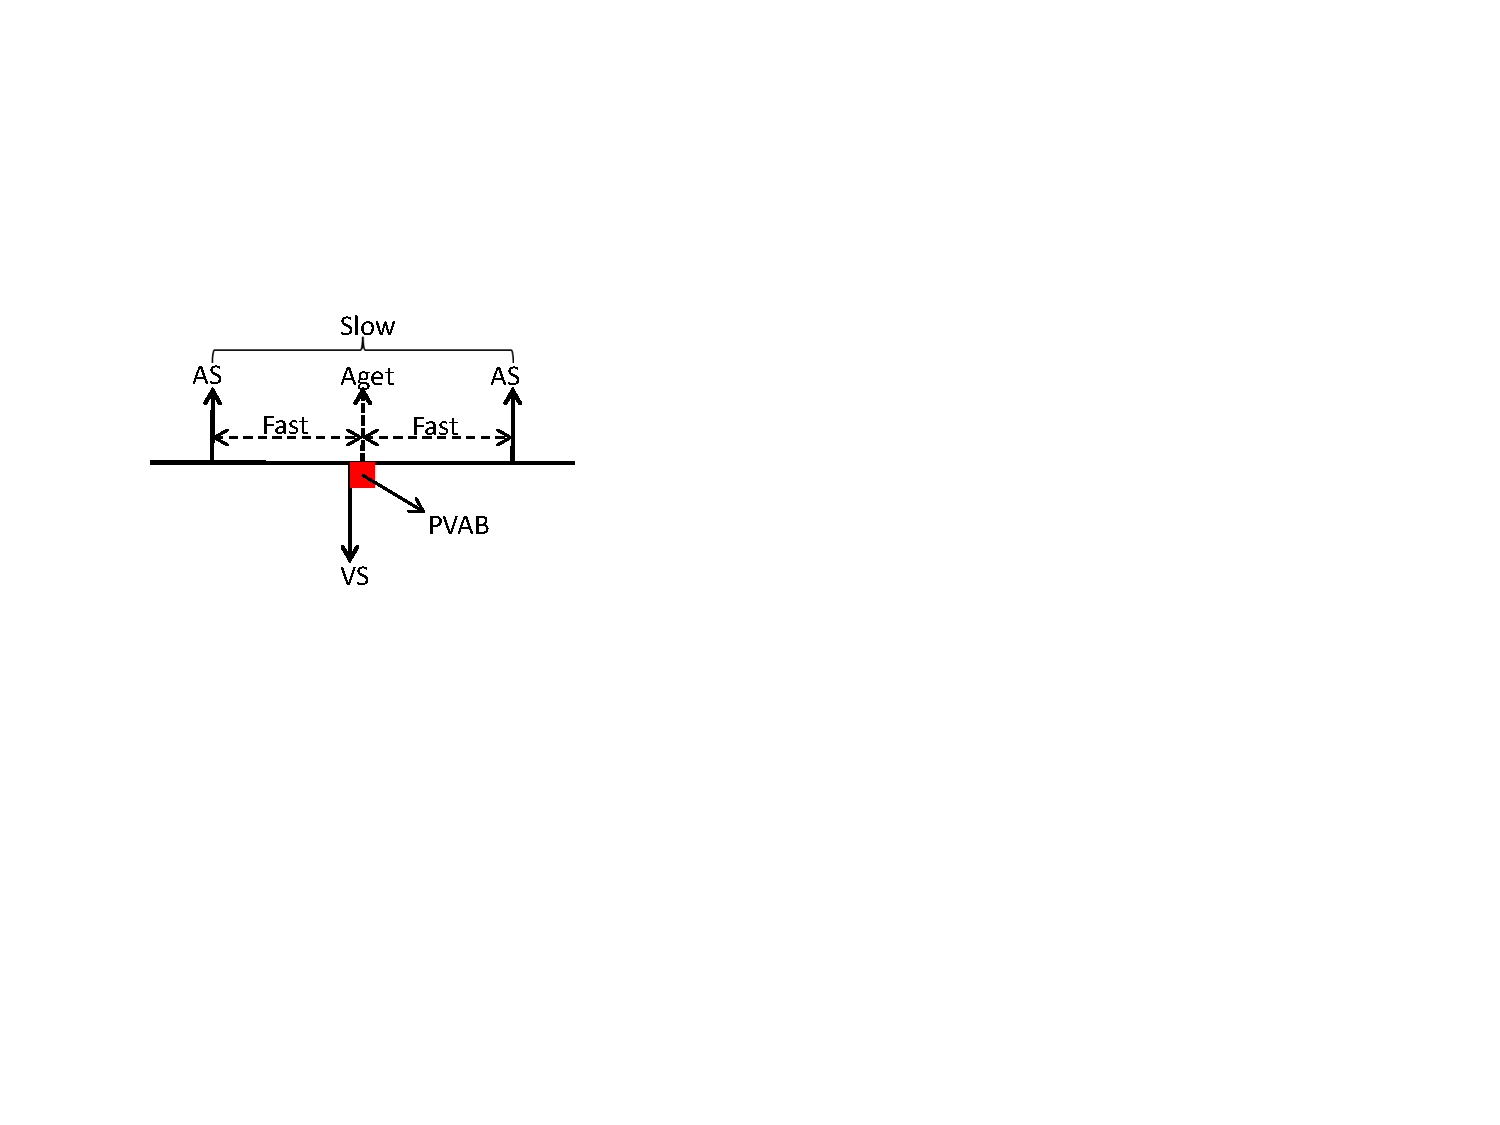
\includegraphics[width=0.2\textwidth]{figs/liveness.pdf}
			\label{fig:liveness}
		}
		\vspace{-10pt}
	\caption{(a) Safety Violation: VP is delayed due to the reset of timer during mode-switch, (b) Correctness Violation: The blocking period may block some atrial events, turning two \emph{Fast} events to one \emph{Slow} event \cite{TACAS12}}
\vspace{-20pt}
\end{figure} 


\chapter{Closed-loop Model Simulation/Testing}
\begin{itemize}
	\item What are the limitations of model checking?
    \item How can simulation complement that?
\end{itemize}

\section{Crosstalk}
Oversensing is a general term for inappropriate sensing caused by noise or far-field signals. It's very common among pacemaker malfunctions and it may result in failure to pace, competitive pacing and inappropriate therapy. Crosstalk is a special case for oversensing which occurs when the pacemaker stimulus in one chamber is sensed in the other chamber. It happens when two leads are close to each other or pacing signal in the other chamber is too strong. It is common that the ventricular lead is placed in the right ventricle outflow tract, which is close to the atrium. \figref{crosstalk}(a) shows simulated EGMs from a patient with bradycardia and complete heart block. During atrial pacing (AP), the pacing signal is sensed by the ventricular lead 53 ms after the AP. (Marker 1) It is treated as ventricular sense (VS) signal and thus inhibit the subsequent ventricular pacing (VP). This is indicated by no QRS-wave in the ECG channel. (Marker 2) For a patient with complete heart block this will cause dangerous ventricular asystole.  

Increasing the sensing threshold of the ventricular channel can prevent false sensing. In \figref{crosstalk}(b), the small signals in ventricular EGM are ignored and ventricular pacing are successfully delivered. 
\begin{figure*}[!t]
\center
\vspace{-10pt}
		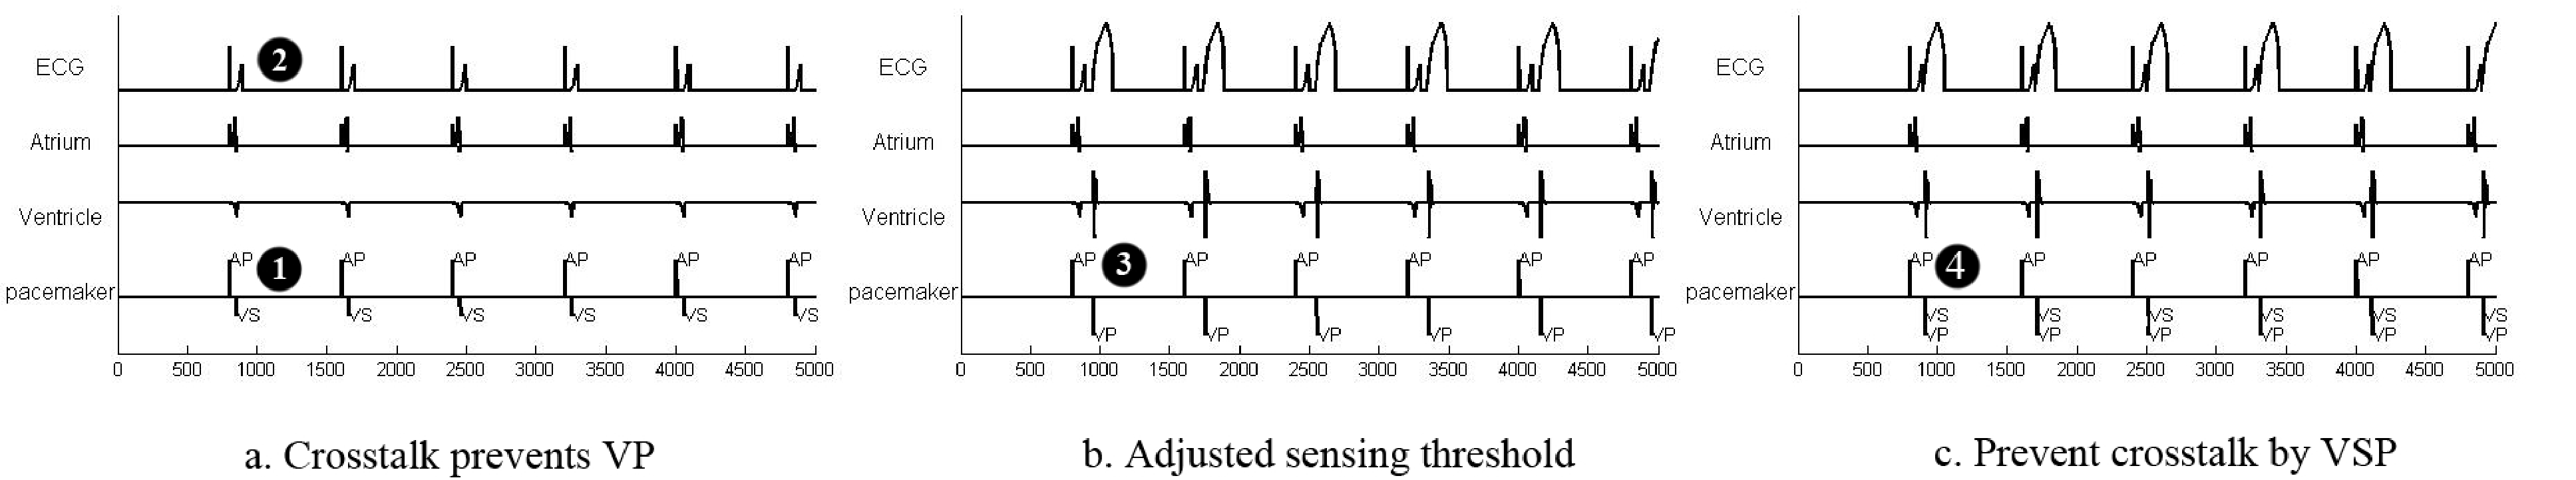
\includegraphics[width=\textwidth]{figs/crosstalk_all.pdf}
\vspace{-20pt}
\caption{Crosstalk between pacemaker leads with high sensitivity in the ventricle, adjusted sensitivity and ventricular safety pacing}
\label{fig:crosstalk}
\vspace{-15pt}
\end{figure*}
\section{Lead Displacement}
